 \documentclass{beamer}

%\usecolortheme[RGB={170,130,220}]{structure}
\setbeamertemplate{items}[ball]
\setbeamertemplate{blocks}[rounded][shadow=true]
%\beamertemplateshadingbackground{yellow!15}{magenta!15}
\usetheme{Singapore}

\usepackage{amsmath, amsthm, amssymb, enumerate, natbib}
\usepackage{graphicx, epsfig}
\usepackage{setspace}
\usepackage{color}
\usepackage{subfigure}

\definecolor{darkgreen}{rgb}{0,0.4,0}
\definecolor{cgreen}{rgb}{0,0.5,0}
\definecolor{darkblue}{rgb}{0,0,0.6}
\definecolor{darkred}{rgb}{0.7,0,0.1}
\definecolor{lessdarkgreen}{rgb}{0.2,0.5,0}
\definecolor{darkerred}{rgb}{0.5,0.1,0.05}
\definecolor{lessdarkred}{rgb}{0.8,0,0}
\definecolor{purple}{rgb}{0.8,.0,0.9}
\definecolor{darkpurple}{rgb}{0.45,.0,1.0}
\definecolor{darkerpurple}{rgb}{0.5,.2,.9}
\definecolor{brightred}{rgb}{1,0,0}


\mode<presentation> {
  \usetheme{Singapore}
  % or ...

  \setbeamercovered{transparent}
  % or whatever (possibly just delete it)
}

\usepackage[english]{babel}
\usepackage[latin1]{inputenc}
\usepackage{times}
\usepackage[T1]{fontenc}
\usepackage{framed}

\newtheorem{proposition}[theorem]{Proposition}
\theoremstyle{definition}
\newtheorem{remark}[theorem]{Remark}
\newtheorem{algorithm}[theorem]{Algorithm}

\begin{document}


\title{\LARGE{Analyzing Flow-Cytometry Count Data with Regression Mixtures}}

\author{\large{\textbf{Amit Meir}} \\ \emph{University of Washington} \\ \vspace{1 cm} Joint work with \\ \vspace{0.1 cm} \textbf{Raphael Gottardo} and \textbf{Greg Finak} 
\\ \emph{Hutchinson Cancer Research Center}}


\vspace{1 cm}

%%%%%%%%%%%%%%%%%%%%%%%%%%%%%%%%%%%%%%%%%

\begin{frame}[plain]
  \titlepage
\end{frame}


%%%%%%%%%%%%%%%%%%%%%%%%%%%%%%%%%%%%%%%%%%%%%%%

\begin{frame}
\frametitle{Outline}
\begin{enumerate}
\item \textbf{Flow-Cytometry - a Refresher}
	\begin{itemize}
	\item Flow Cytometry?????
	\item A model in need of a better name than flowReMix.
	\end{itemize}
\vspace{0.3 cm}
\item \textbf{RV144}
	\begin{itemize}
	\item Inferred Graphical Model
	\item Cumulative Response Measures.
	\end{itemize}
\vspace{0.3 cm}
\item \textbf{HVTN505}:
	\begin{itemize}
	\item Graphical Model.
	\item Correlates for Infection Status (Clinical Outcome).
	\item Breadth/Polyfunctionality Anaysis.
	\end{itemize}
	\vspace{0.3 cm}
\item \textbf{CHMI Study}
	\begin{itemize}
	\item Longitudal Data.
	\item Enrichment Analysis.
	\end{itemize}
\end{enumerate}
\end{frame}

%%%%%%%%%%%%%%%%%%%%%%%%%%%%%%%%%%%%%%%

\begin{frame}
\frametitle{The RV144 HIV Vaccine Trial}
\begin{center}
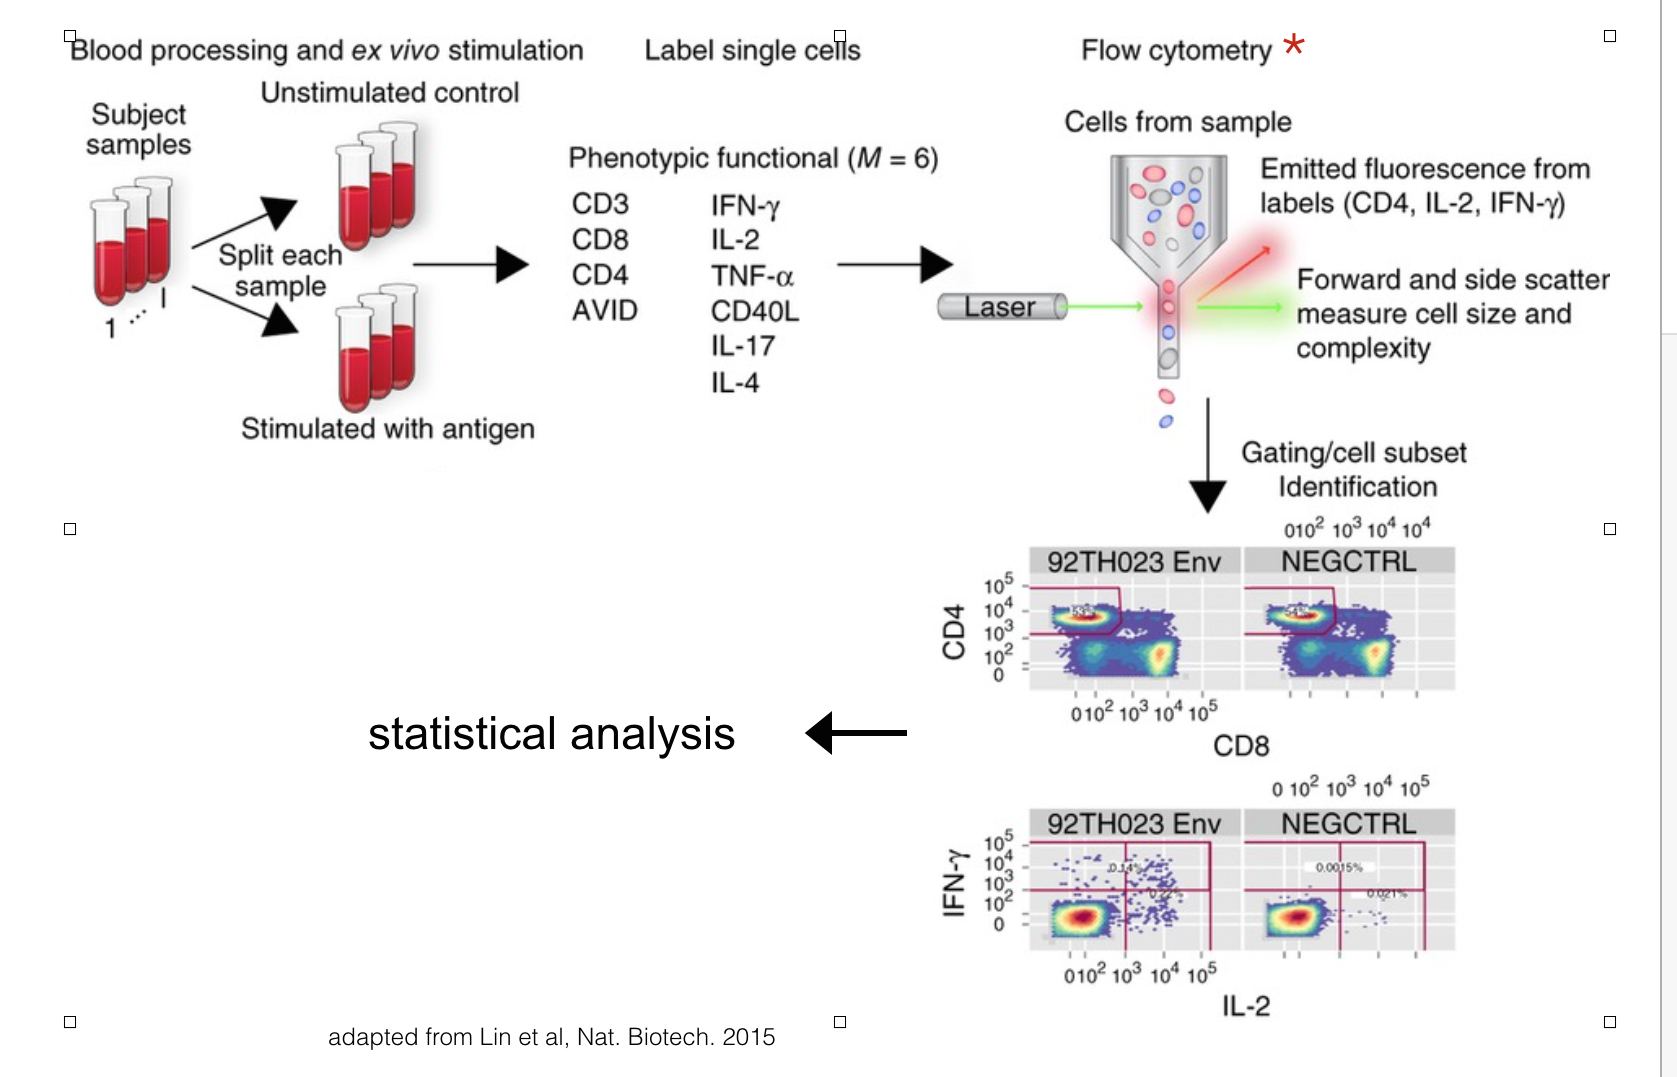
\includegraphics[scale=0.4]{figures/flowcytintro}
\end{center}
\end{frame}

%%%%%%%%%%%%%%%%%%%%%%%%%%%%%%%%%%%%%%%%%%%%%%%

\begin{frame}
\frametitle{The RV144 HIV Vaccine Trial}
\begin{figure}[]
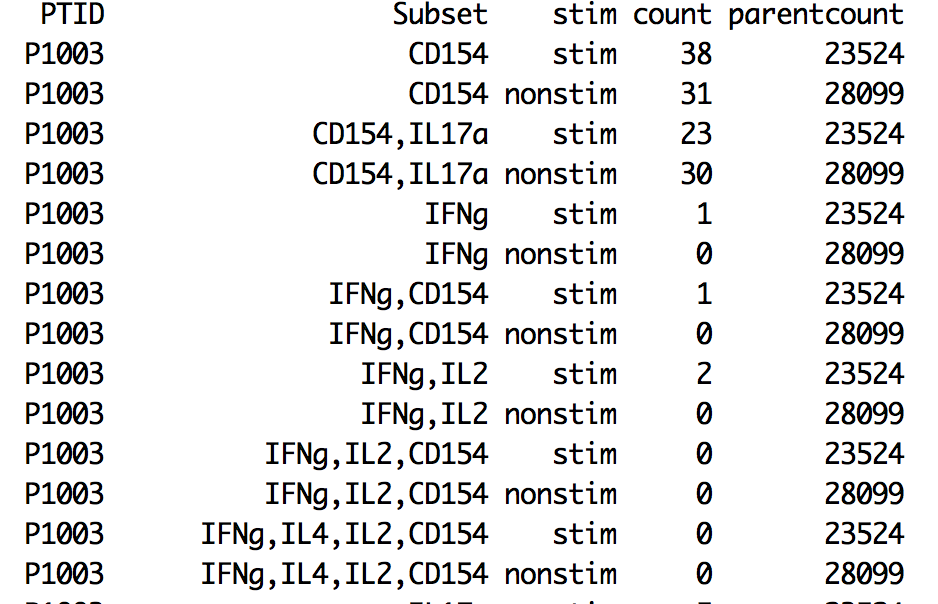
\includegraphics[width=12 cm]{figures/datasetExample} \caption{}
\end{figure}
\end{frame}

%%%%%%%%%%%%%%%%%%%%%%%%%%%%%%%%%%%%%%%%%%%%%%%

\begin{frame}
\frametitle{Marginal Counts for RV144}
\begin{center}
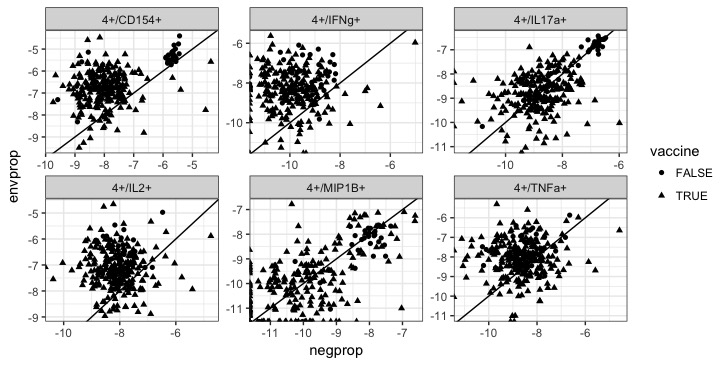
\includegraphics[scale=0.4]{figures/marginalScatterNoPost}
\end{center}
\end{frame}

%%%%%%%%%%%%%%%%%%%%%%%%%%%%%%%%%%%%%%%%

\begin{frame}
\frametitle{The Beta-Binomial Distribution}
The Beta-Binomial distribution is a type of over dispersed Binomial distribution.
$$
p \sim Beta(\mu M, (1 - \mu) M)
$$$$
y \sim Bin(N, p)
$$

\pause
\vspace{0.5 cm}
$$
E(\bar{y}) = \mu
$$$$
Var(\bar{y}) = \frac{\mu(1- \mu)}{N} + \frac{\mu(1 - \mu)}{M + 1}
$$
\end{frame}

%%%%%%%%%%%%%%%%%%%%%%%%%%%%%%%%%%%%%%%%%%%%%%%

\begin{frame}
\frametitle{A Random Intercept Model}
\begin{framed}
Indexing: \textbf{i}-subject, \textbf{t}- subsample, \textbf{j}- subset.
\end{framed}

$$
\nu_i \sim N(0, \Sigma),
$$$$
\text{logit}(\mu_{ijt}) = X_{ijt} \beta_j + \nu_{ij} ,
$$$$
y_{ijt} \sim \text{Beta-Binomial}(N_{it}, \mu_{ijt}, M_j) ,
$$
\end{frame}

%%%%%%%%%%%%%%%%%%%%%%%%%%%%%%%%%%%%%%%%%%%%%%%

\begin{frame}
\frametitle{An Individual Response Model}
\begin{framed}
Indexing: \textbf{i}-subject, \textbf{t}- subsample, \textbf{j}- subset.
\end{framed}

We want to allow for individual subjects/cell-subsets to have differential response to stimulation. 
$$
\text{logit}(\mu_{ijt}) = X_{ijt} \beta + T_{ijt}\tau_{ij} + \nu_{ij} ,
$$$$
\tau_{ij} = 
\begin{cases}
\tau_j & \text{response in }\{i,j\} \\
0 & \text{no response}
\end{cases}.
$$
\end{frame}

%%%%%%%%%%%%%%%%%%%%%%%%%%%%%%%%%%%%%%%%%%%%%%%]

\begin{frame}
\frametitle{A Markov Random Field Model}
\begin{framed}
Indexing: \textbf{i}-subject, \textbf{t}- stimulation, \textbf{j}- subset.
\end{framed}

Denote cluster (Response) by a $z \in \{0,1\}^{p}$ vector with $1$ indicating a responsive subset.
\pause
\vspace{0.3 cm}

We assume an Ising model for the dependence structure between subsets:
$$
P(z) \propto \sum_{j=1}^{p} z_{j} \theta_j + \sum_{u\neq v} z_{u} z_{v} \theta_{uv},
$$$$
P(z_{j} = 1| z_{-j}) = \theta_{j} + \sum_{u\neq j } z_u \theta_{uj}.
$$

\pause
\vspace{0.3 cm}
We can induce sparsity through an $\ell_1$ penalty.

\end{frame}

%%%%%%%%%%%%%%%%%%%%%%%%%%%%%%%%%%%%%%%%%%%%%%%]

\begin{frame}
\frametitle{A Hidden Markov Random Field Model}
\begin{framed}
Indexing: \textbf{i}-subject, \textbf{t}- stimulation, \textbf{j}- subset.
\end{framed}

$$
\nu_i \sim N(0, \Sigma),
$$$$
z_i \sim \text{Ising}(\theta).
$$$$
\text{logit}(\mu_{ijt}) = X_{ijt} \beta_j + T_{ijt}\tau_j(z_i) + \nu_{ij} ,
$$$$
y_{ijt} \sim \text{Beta-Binomial}(N_{it}, \mu_{ijt}, M_j) ,
$$
\end{frame}

%%%%%%%%%%%%%%%%%%%%%%%%%%%%%%%%%%%%%%%%%%%%%%%]

\begin{frame}
\frametitle{The RV144 HIV Vaccine Trial}
\begin{itemize}
\item \textbf{262 Subjects}
	\begin{itemize}
	\item 226 Cases
	\item 36 Controls
	\end{itemize}
\vspace{0.2 cm}
\item \textbf{2 Types of stimulus} 
	\begin{itemize}
	\item HIV protein
	\item Negative control
	\end{itemize}
\vspace{0.2 cm}
\item \textbf{23 CD4 Cell-Subsets.} 
\end{itemize}
\end{frame}

%%%%%%%%%%%%%%%%%%%%%%%%%%%%%%%%%%%%%%%%%%%%%%%

\begin{frame}
\frametitle{RV144 - Booleans Dataset}
\begin{figure}[]
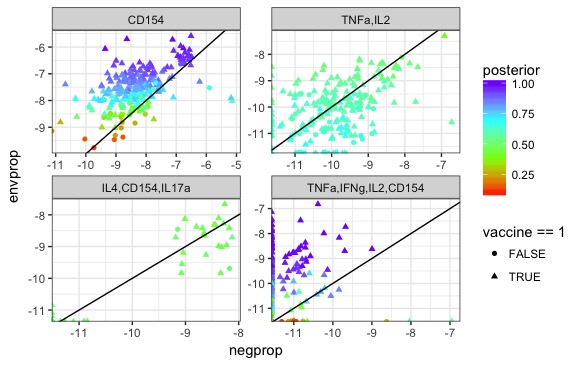
\includegraphics[width=12 cm]{figures/booleansScatterLess} 
\end{figure}
\end{frame}

%%%%%%%%%%%%%%%%%%%%%%%%%%%%%%%%%%%%%%%%%%%%%%%]

\begin{frame}
\frametitle{RV144 - Booleans Dataset}
\begin{figure}[]
\includegraphics[width=12 cm]{figures/BooleansROCless}
\end{figure}
\end{frame}

%%%%%%%%%%%%%%%%%%%%%%%%%%%%%%%%%%%%%%%%%%%%%%%]

\begin{frame}
\frametitle{RV144 - Booleans Dataset}
\begin{figure}[]
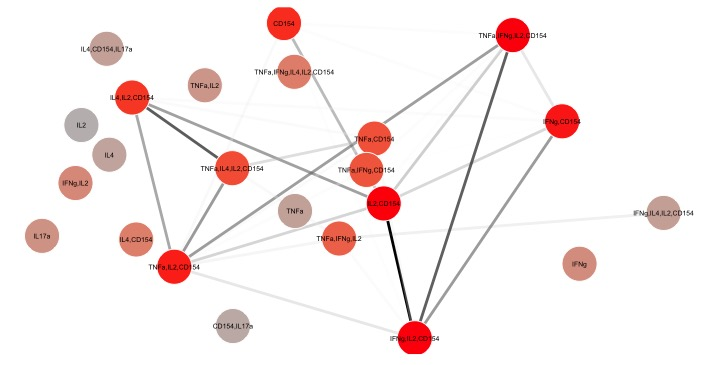
\includegraphics[width= 10.5 cm]{figures/booleansNetworkAUC} 
\caption{Estimated Ising Model - Red marks AUC}
\end{figure}
\end{frame}

%%%%%%%%%%%%%%%%%%%%%%%%%%%%%%%%%%%%%%%%%%%%%%%]

\begin{frame}
\frametitle{A Better Way to Estimate the Graphical Model?}
The graph output by the procedure is an average of the graph estimated in several iterations. 
\begin{itemize}
	\item Not as sparse as we would like...
	\item How sure are we of existence of an edge?
\end{itemize}

\pause
\vspace{1 cm}
Possible solution, stability selection:
\begin{itemize}
	\item Draw samples from the posterior response distribution.
	\item Fit a Graphical Model.
	\item \textbf{Repeat}
\end{itemize}
Compute the proportion of estimated models in which an edge has been observed.
\end{frame}

%%%%%%%%%%%%%%%%%%%%%%%%%%%%%%%%%%%%%%%%%%%%%%%]

\begin{figure}[]
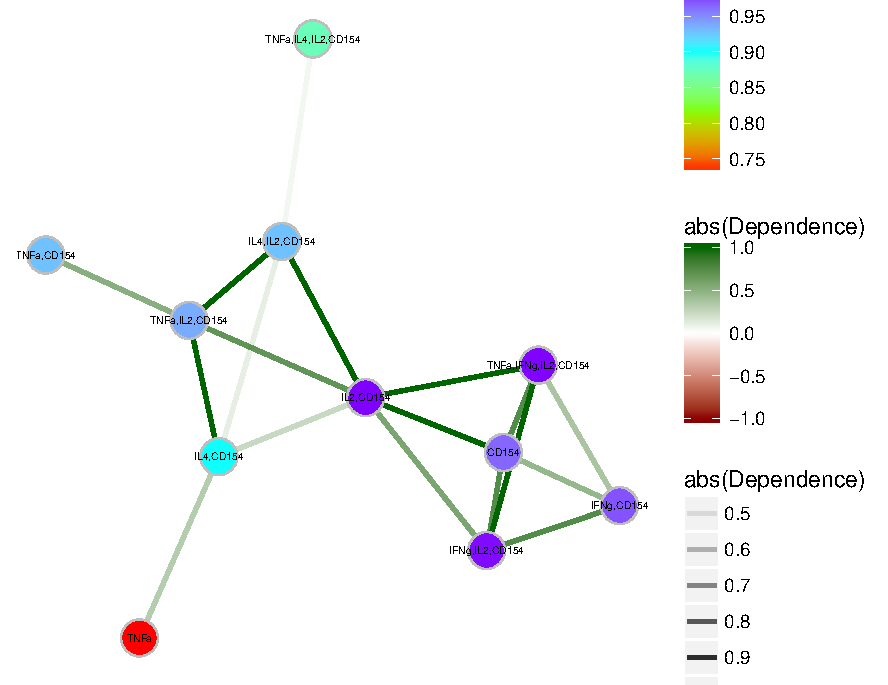
\includegraphics[width=11 cm]{figures/RV144stability}
\end{figure}

%%%%%%%%%%%%%%%%%%%%%%%%%%%%%%%%%%%%%%%%%%%%%%%]

\begin{frame}
\frametitle{Aggregating Subject Response}
So far we have used posterior samples to:
\begin{itemize}
\item Identify responsive cell-subsets.
\item Infer Dependence Structures. 
\end{itemize}

\pause
\vspace{0.5 cm}
How can we identify (or rank) responsive subjects?
\begin{itemize}
\item Responsive subject = 1 responsive subset? 2? 3?...
\item How about stochastic ordering? 
$$
F \preceq G \;\; \Leftrightarrow \;\; G(x) \leq F(x) \;\; \forall x
$$
\end{itemize}

\vspace{0.3 cm}
\pause
\textbf{We can compute a posterior CDF for \# of responses for each subject!}
\end{frame}

%%%%%%%%%%%%%%%%%%%%%%%%%%%%%%%%%%%%%%%%%%%%%%%]

\begin{frame}
\frametitle{Posterior CDFs for Response}
\begin{figure}[]
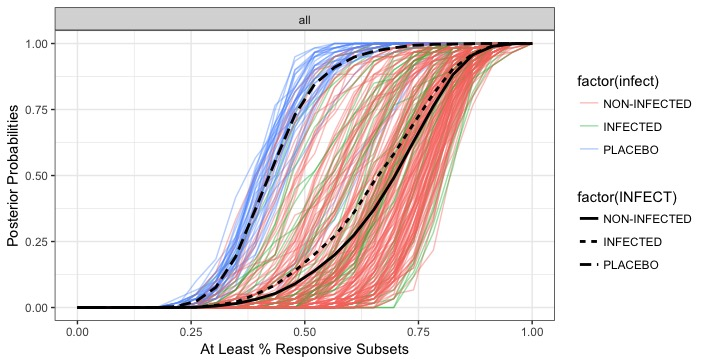
\includegraphics[width=11 cm]{figures/RV144CDFs}
\end{figure}
There is a stochastic ordering between outcome categories! (p-value $\approx 0.035$)
\end{frame}

%%%%%%%%%%%%%%%%%%%%%%%%%%%%%%%%%%%%%%%%%%%%%%%]

\begin{frame}
\frametitle{A Functionality Score}
We compute the area under the curve as an individual functionality measure. 
\begin{figure}[]
\includegraphics[width=8 cm]{figures/rv144funcroc}
\end{figure}
\end{frame}

%%%%%%%%%%%%%%%%%%%%%%%%%%%%%%%%%%%%%%%%%%%%%%%]

\begin{frame}
\frametitle{The HVTN 505 Vaccine Trial}
\begin{itemize}
\item \textbf{238 Subjects}
	\begin{itemize}
	\item 189 Cases
	\item 49 Controls
	\end{itemize}
\vspace{0.2 cm}
\item \textbf{5 Types of stimulus} 
	\begin{itemize}
	\item 4 types of HIV proteins (ENV, GAG, POL, NEF).
	\item Negative control.
	\end{itemize}
\vspace{0.2 cm}
\item \textbf{52 Cell Subsets}
	\begin{itemize}
	\item $25$ CD4 cells.
	\item $27$ CD8 cells.
	\end{itemize} 
\end{itemize}
\end{frame}

%%%%%%%%%%%%%%%%%%%%%%%%%%%%%%%%%%%%%%%%%%%%%%%]

\begin{frame}
\frametitle{Analysis Goals}
\begin{itemize}
\item \textbf{Problem:} We are interested in identifying response in Subsets X Protein pairs. 

\pause
\vspace{0.5 cm}
\item \textbf{Solution:} Define each combination of Subset X Protein as a cell-subset.
	\begin{itemize}
	\item Overall 184 subsets with non-negligible counts. 
	\end{itemize}

\vspace{0.5 cm}
\item Dependence structures should (and do!) sort themselves out.

\pause
\vspace{0.5 cm}
\item Include covariates?
\end{itemize}
\end{frame}

%%%%%%%%%%%%%%%%%%%%%%%%%%%%%%%%%%%%%%%%%%%%%%%]

\begin{frame}
\frametitle{Inferred Graph}
\begin{figure}[]
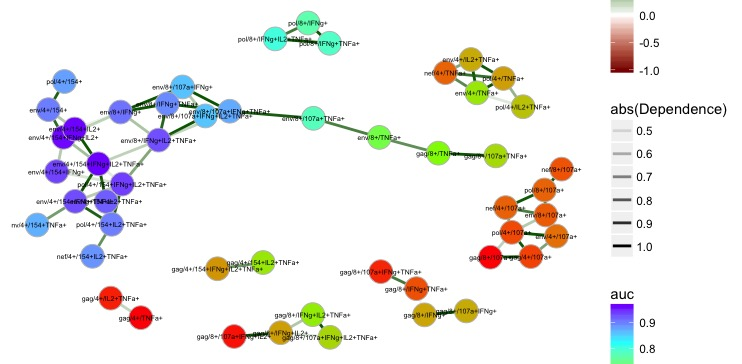
\includegraphics[width=12 cm]{figures/HVTNnetworkAll}
\end{figure}
\end{frame}

%%%%%%%%%%%%%%%%%%%%%%%%%%%%%%%%%%%%%%%%%%%%%%%]

\begin{frame}
\frametitle{Inferred Graph}
\begin{figure}[]
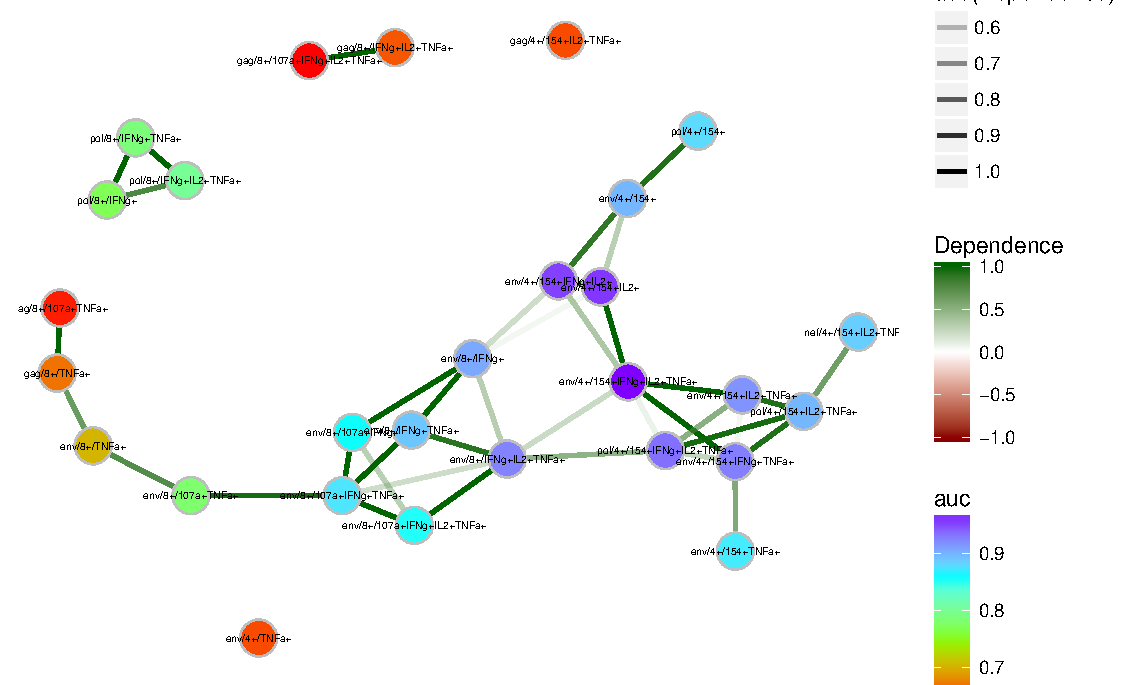
\includegraphics[width=11 cm]{figures/HVTNgraphSigPdf}
\end{figure}
\end{frame}

%%%%%%%%%%%%%%%%%%%%%%%%%%%%%%%%%%%%%%%%%%%%%%%]

\begin{frame}
\frametitle{Correlates for Infection-Status}
As we have done for the RV144 dataset, we can correlate response in different cell-subsets with either \textbf{vaccination} status, or \textbf{infection} status.

\begin{center}
\textbf{Top Subsets For Vaccination Status (54 significant)}
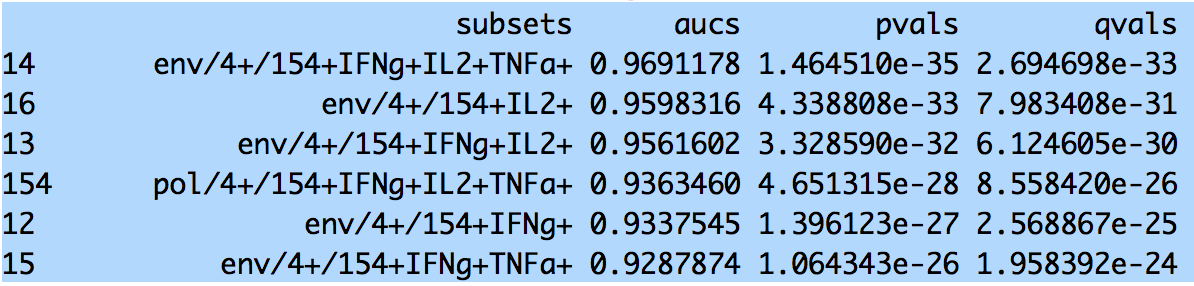
\includegraphics[width=10 cm]{figures/vaccineTable}
\end{center}

\begin{center}
\textbf{Top Subsets For Infection Status (4 significant)}
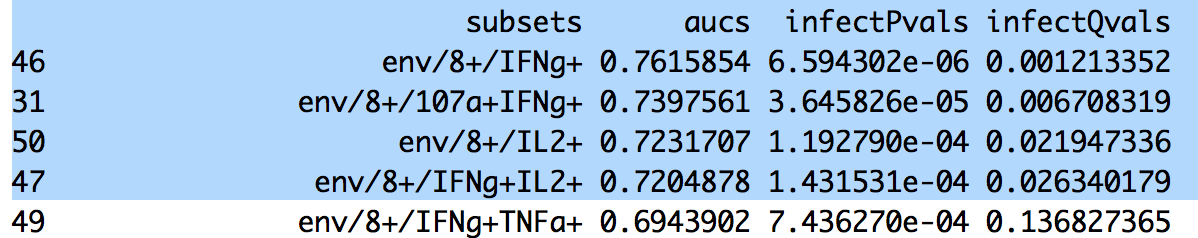
\includegraphics[width=10 cm]{figures/infectionTable}
\end{center}

\end{frame}

%%%%%%%%%%%%%%%%%%%%%%%%%%%%%%%%%%%%%%%%%%%%%%%]

\begin{frame}
\frametitle{Aggregate Measures of Response}
We have many more cell-subsets here, and can ask more interesting questions. Can we think of better aggregate measures?

\vspace{0.2 cm}
\pause
\begin{itemize}
\item \textbf{Polyfunctionality:}
	\begin{itemize}
	\item Polyfunctional cells produce multiple cytokines.
	\item Few, but may play an important role in immunization. 
	\item \textbf{Implication:} Give higher weights to polyfunctional cells.
	\end{itemize}
	
\pause
\vspace{1 cm}
\item \textbf{Breadth:}
	\begin{itemize}
	\item How man stimulations does a subject respond to?
	\item \textbf{Implication:} Give higher weights to first responsive subsets for a given stimulation.
	\end{itemize}
\end{itemize}
\end{frame}

%%%%%%%%%%%%%%%%%%%%%%%%%%%%%%%%%%%%%%%%%%%%%%%]

\begin{frame}
\frametitle{HVTN Polyfunctionality CDFs}
\begin{figure}[]
\includegraphics[width=11 cm]{figures/HVTNpolyOnlyCDF}
\end{figure}
\end{frame}

%%%%%%%%%%%%%%%%%%%%%%%%%%%%%%%%%%%%%%%%%%%%%%%]

\begin{frame}
\frametitle{HVTN Polyfunctionality Score Boxplots}
\begin{figure}
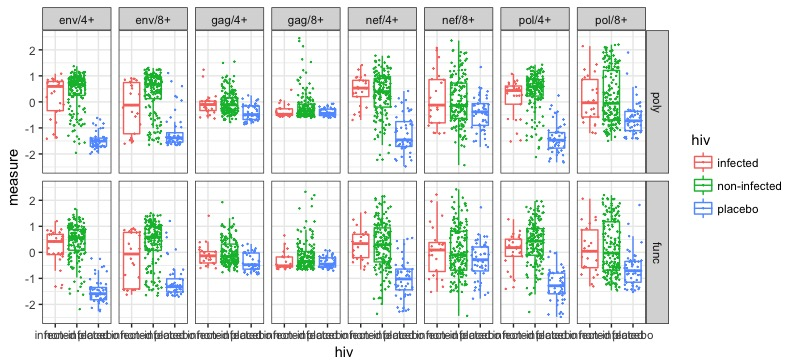
\includegraphics[width=11 cm]{figures/HVTNfuncbox}
\end{figure}
\end{frame}

%%%%%%%%%%%%%%%%%%%%%%%%%%%%%%%%%%%%%%%%%%%%%%%]

\begin{frame}
\frametitle{HVTN Polyfunctionality Score ROCs}
\begin{figure}
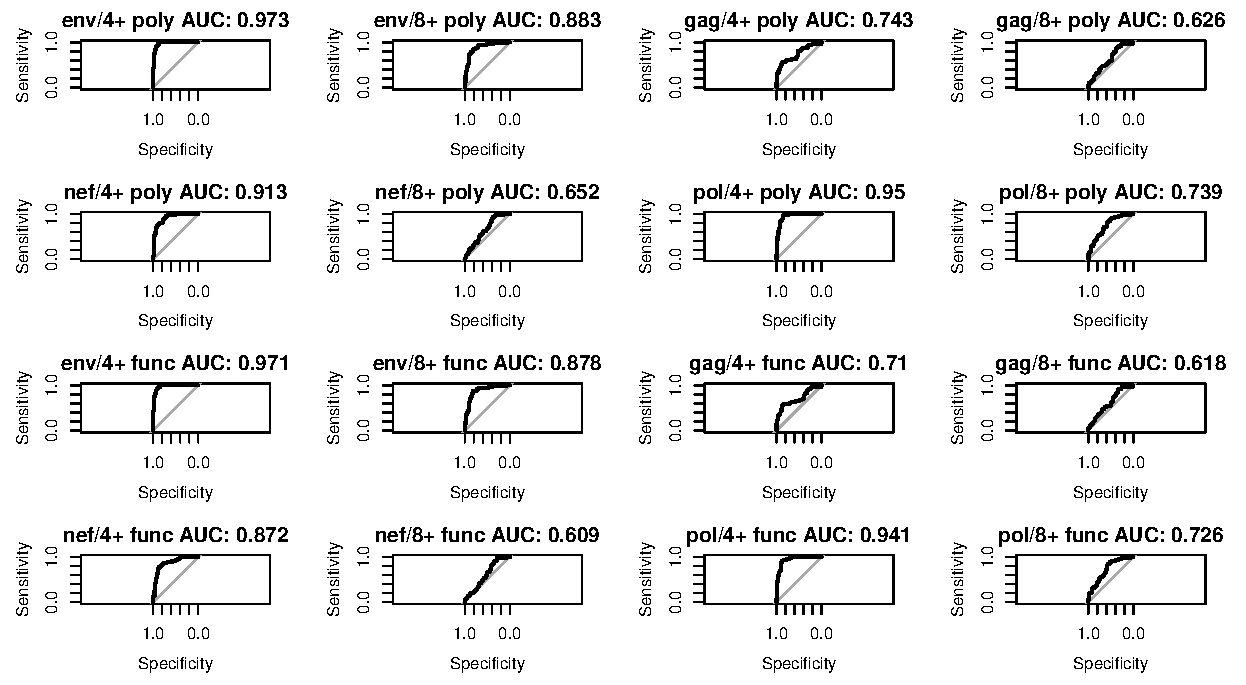
\includegraphics[width=11 cm]{figures/HVTNpolyROC}
\end{figure}
\end{frame}

%%%%%%%%%%%%%%%%%%%%%%%%%%%%%%%%%%%%%%%%%%%%%%%]

\begin{frame}
\frametitle{HVTN Breadth CDFs}
\begin{figure}
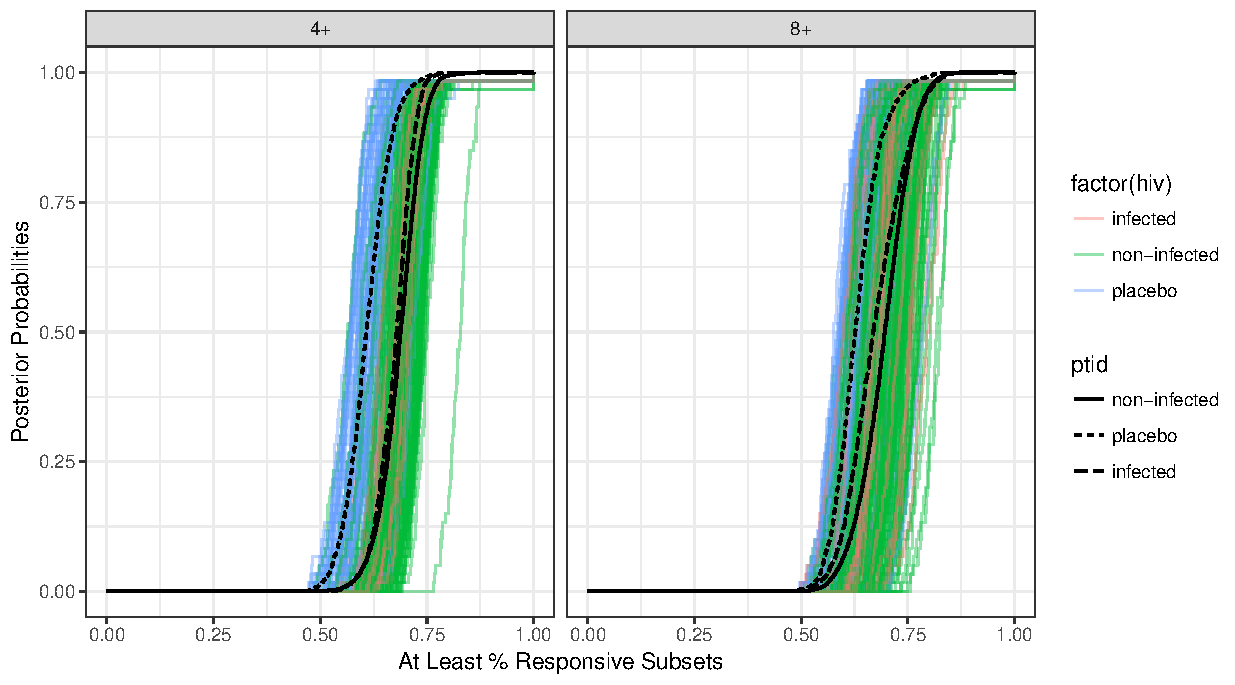
\includegraphics[width=11 cm]{figures/HVTNbreadthCDFs}
\end{figure}
\end{frame}

%%%%%%%%%%%%%%%%%%%%%%%%%%%%%%%%%%%%%%%%%%%%%%%]

\begin{frame}
\frametitle{Breadth - ROC for Infection Study}
\begin{figure}
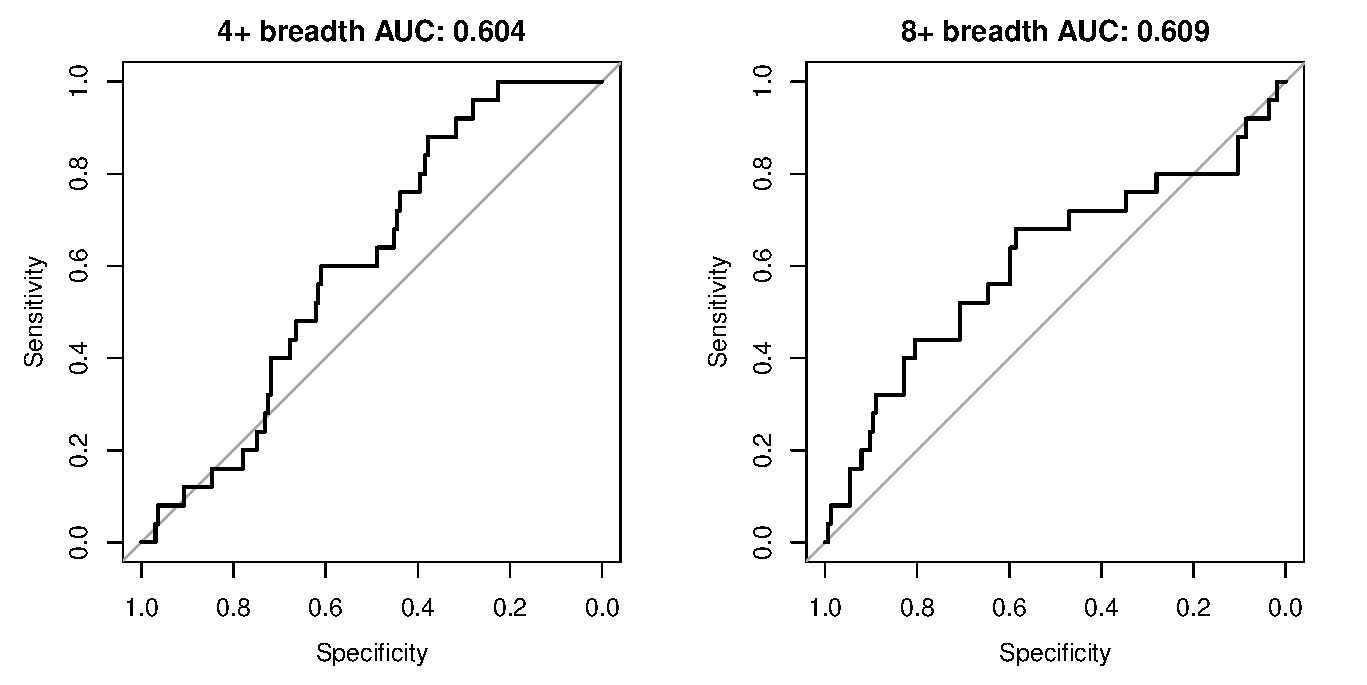
\includegraphics[width=11 cm]{figures/HVTNbreadthROCinfection}
\end{figure}
\textbf{P-value $< 0.05$ for both ROCs}
\end{frame}







\begin{frame}
\frametitle{Controlled Human Malaria Infection Study}
\begin{figure}[]
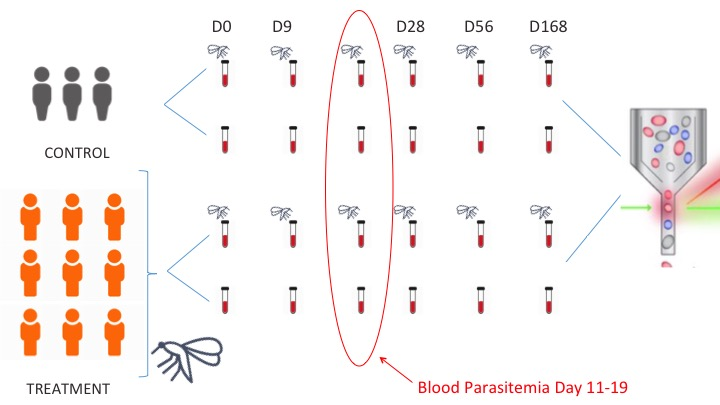
\includegraphics[width=11 cm]{figures/malariaGraphic}
\end{figure}
\end{frame}

%%%%%%%%%%%%%%%%%%%%%%%%%%%%%%%%%%%%%%%%%%%%%%%]

\begin{frame}
\frametitle{Controlled Human Malaria Infection Study}
\begin{itemize}
\item 9 subjects were infected with Malaria.
	\begin{itemize}
	\item +3 controls.
	\end{itemize}
	\vspace{0.75 cm}
	
\item Blood samples were collected at 6 time points.
	\begin{itemize}
	\item Day 0, day 9, blood  parasitemia, Day 28, Day 56, Day 168.
	\end{itemize}
	\vspace{0.75 cm}

\item Two types of stimulation:
	\begin{itemize}
	\item Infected/uninfected blood-cells.
	\end{itemize}
	\vspace{0.75 cm}
	
\item 53 cell subsets.
	\begin{itemize}
	\item (10 types of cytokines in 8 cell-types)
	\end{itemize} 
\end{itemize}
\end{frame}

%%%%%%%%%%%%%%%%%%%%%%%%%%%%%%%%%%%%%%%%%%%%%%%]

\begin{frame}
\frametitle{Controlled Human Malaria Infection Study}
\begin{itemize}
\item  Individuals  who  experience malaria  infections develop  immunity.
	\begin{itemize}
	\item All subject may exhibit response to stimulation.
	\item Even at day 0!
	\item What is the profile of the immune response?
	\end{itemize}
	
\pause
\vspace{0.5 cm}
\item The  immunity is not long lived.
	\begin{itemize}
	\item We might expect to see a rise in response during experiment.
	\item How fast does the response return to baseline?
	\end{itemize}
\end{itemize}
\end{frame}

%%%%%%%%%%%%%%%%%%%%%%%%%%%%%%%%%%%%%%%%%%%%%%%]

\begin{frame}
\frametitle{Controlled Human Malaria Infection Study}
\begin{figure}[]
\includegraphics[width=12 cm]{figures/fourPlusSmoothedNarrow} \caption{CD4 Helper Cells}
\end{figure}
\end{frame}

%%%%%%%%%%%%%%%%%%%%%%%%%%%%%%%%%%%%%%%%%%%%%%%]

\begin{frame}
\frametitle{FDR Adjusted p-values for CHMI Study}
Standard errors for significance tests computed using Jackknife. 
\vspace{0.4 cm}

% latex table generated in R 3.3.2 by xtable 1.8-2 package
% Thu Feb 23 03:35:46 2017
\begin{table}[ht]
\centering
\scalebox{0.65}{
\begin{tabular}{rlllllrll}
  \hline
 & 4+ & 4+/CXCR5+ & 56+dim & 56+hi & 8+ & 8+/CXCR5+ & NK T cells & PD-1+ \\ 
  \hline
154+ & \colorbox{yellow}{0.029} & \colorbox{yellow}{0.004} &  &  & 0.103 & 0.75 & \colorbox{yellow}{0.006} & \colorbox{yellow}{0.024} \\ 
  CCR7+ & 0.649 & 0.996 &  &  & 0.596 & 0.51 &  &  \\ 
  CD45A+ & 0.575 & 0.307 &  &  & 0.543 & 0.54 &  &  \\ 
  IFNg+ & \colorbox{yellow}{0.001} & \colorbox{yellow}{0.006} & \colorbox{yellow}{0.065} & 0.146 & \colorbox{yellow}{0.001} &  & \colorbox{yellow}{0.052} & \colorbox{yellow}{0.097} \\ 
  IL2+ & \colorbox{yellow}{0} & \colorbox{yellow}{0.005} &  &  & 0.119 & 0.56 & 0.321 & \colorbox{yellow}{0.052} \\ 
  IL21+ & 0.676 & 0.649 & 0.751 & 0.589 & 0.649 &  & 0.71 &  \\ 
  IL4+ & 0.12 & 0.543 &  & 0.751 & 0.649 &  & 0.583 &  \\ 
  TNFa+ & \colorbox{yellow}{0} & \colorbox{yellow}{0.001} & 0.261 & 0.309 & 0.276 &  & \colorbox{yellow}{0.053} & \colorbox{yellow}{0.09} \\ 
  GzB+ & 0.583 &  & 0.511 & \colorbox{yellow}{0.001} & 0.589 &  & 0.596 &  \\ 
  PD-1+ & 0.751 &  &  &  & 0.596 & 0.83 &  &  \\ 
   \hline
\end{tabular}}
\end{table}
\end{frame}

%%%%%%%%%%%%%%%%%%%%%%%%%%%%%%%%%%%%%%%%%%%%%%%]

\begin{frame}
\frametitle{Controlled Human Malaria Infection Study}
\begin{figure}[]
\includegraphics[width=13 cm]{figures/MalariaSignificantAt10} \caption{Significant Subsets}
\end{figure}
\end{frame}

%%%%%%%%%%%%%%%%%%%%%%%%%%%%%%%%%%%%%%%%%%%%%%%]

\begin{frame}
\frametitle{Enrichment Analysis and Valid Ad-Hoc Testing}
The data seems to suggest testing for elevated response after parasitemia. 
\vspace{0.4 cm}

This effect may be small, and was identified based on the data.

\pause
\vspace{0.4 cm}
Possible Solution:
\begin{itemize}
\item Test enrichments (groups of cells) to obtain more power. 
\item Perform a post-selection test for subsets within enrichments that pass a threshold.
\end{itemize}

\pause
\vspace{0.4 cm}
We test:
\begin{itemize}
\item \textbf{Enrichments:} Th1, Th2, Gzb.
\item \textbf{Hypotheses:} Overall effect, elevated response at 28, 56, 168.
\end{itemize}
\end{frame}

%%%%%%%%%%%%%%%%%%%%%%%%%%%%%%%%%%%%%%%%%%%%%%%]

\begin{frame}
\frametitle{Controlled Human Malaria Infection Study}
\begin{figure}[]
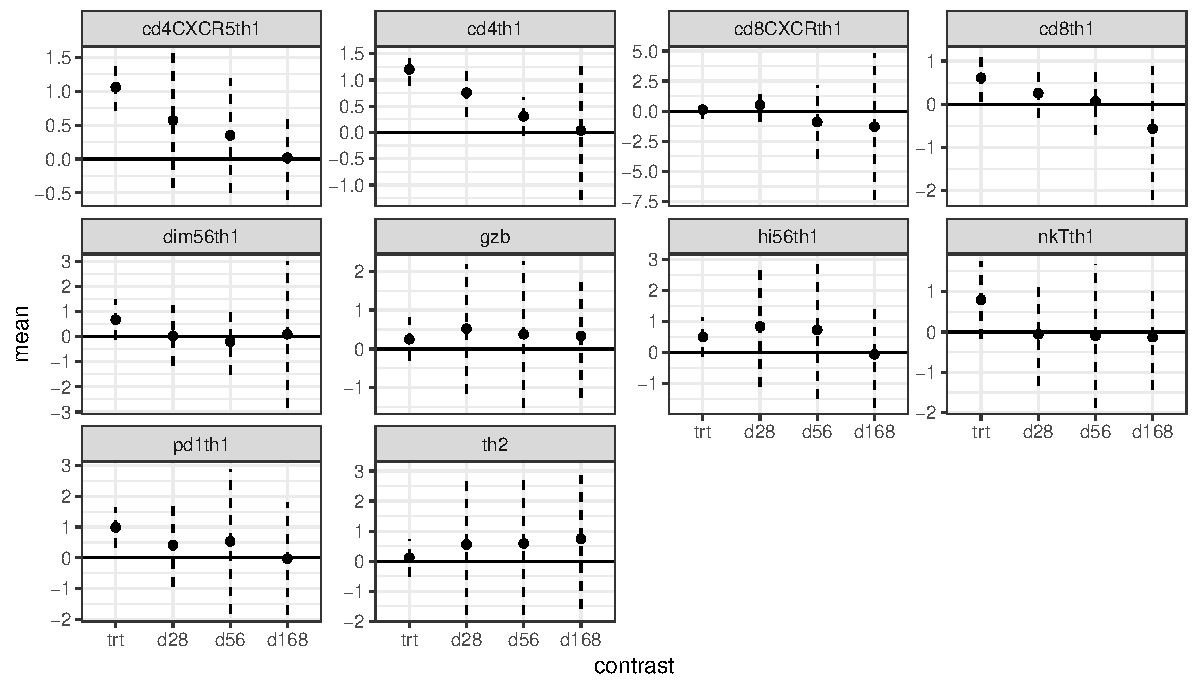
\includegraphics[width=10 cm]{figures/malariaAggregates} 
\end{figure}
\end{frame}

%%%%%%%%%%%%%%%%%%%%%%%%%%%%%%%%%%%%%%%%%%%%%%%]

\begin{frame}
\frametitle{Controlled Human Malaria Infection Study}
\begin{figure}[]
\includegraphics[width=10 cm]{figures/malariapost} \end{figure}
\end{frame}

%%%%%%%%%%%%%%%%%%%%%%%%%%%%%%%%%%%%%%%%%%%%%%%]

\begin{frame}
\begin{center}
\huge{Thank you!}

\vspace{2 cm}
\LARGE{Questions?}

\vspace{1cm}
\large{AmitMeir@uw.edu}
\end{center}
\end{frame}


\end{document}